
% Default to the notebook output style

    


% Inherit from the specified cell style.




    
\documentclass[11pt]{article}

    
    
    \usepackage[T1]{fontenc}
    % Nicer default font (+ math font) than Computer Modern for most use cases
    \usepackage{mathpazo}

    % Basic figure setup, for now with no caption control since it's done
    % automatically by Pandoc (which extracts ![](path) syntax from Markdown).
    \usepackage{graphicx}
    % We will generate all images so they have a width \maxwidth. This means
    % that they will get their normal width if they fit onto the page, but
    % are scaled down if they would overflow the margins.
    \makeatletter
    \def\maxwidth{\ifdim\Gin@nat@width>\linewidth\linewidth
    \else\Gin@nat@width\fi}
    \makeatother
    \let\Oldincludegraphics\includegraphics
    % Set max figure width to be 80% of text width, for now hardcoded.
    \renewcommand{\includegraphics}[1]{\Oldincludegraphics[width=.8\maxwidth]{#1}}
    % Ensure that by default, figures have no caption (until we provide a
    % proper Figure object with a Caption API and a way to capture that
    % in the conversion process - todo).
    \usepackage{caption}
    \DeclareCaptionLabelFormat{nolabel}{}
    \captionsetup{labelformat=nolabel}

    \usepackage{adjustbox} % Used to constrain images to a maximum size 
    \usepackage{xcolor} % Allow colors to be defined
    \usepackage{enumerate} % Needed for markdown enumerations to work
    \usepackage{geometry} % Used to adjust the document margins
    \usepackage{amsmath} % Equations
    \usepackage{amssymb} % Equations
    \usepackage{textcomp} % defines textquotesingle
    % Hack from http://tex.stackexchange.com/a/47451/13684:
    \AtBeginDocument{%
        \def\PYZsq{\textquotesingle}% Upright quotes in Pygmentized code
    }
    \usepackage{upquote} % Upright quotes for verbatim code
    \usepackage{eurosym} % defines \euro
    \usepackage[mathletters]{ucs} % Extended unicode (utf-8) support
    \usepackage[utf8x]{inputenc} % Allow utf-8 characters in the tex document
    \usepackage{fancyvrb} % verbatim replacement that allows latex
    \usepackage{grffile} % extends the file name processing of package graphics 
                         % to support a larger range 
    % The hyperref package gives us a pdf with properly built
    % internal navigation ('pdf bookmarks' for the table of contents,
    % internal cross-reference links, web links for URLs, etc.)
    \usepackage{hyperref}
    \usepackage{longtable} % longtable support required by pandoc >1.10
    \usepackage{booktabs}  % table support for pandoc > 1.12.2
    \usepackage[inline]{enumitem} % IRkernel/repr support (it uses the enumerate* environment)
    \usepackage[normalem]{ulem} % ulem is needed to support strikethroughs (\sout)
                                % normalem makes italics be italics, not underlines
    

    
    
    % Colors for the hyperref package
    \definecolor{urlcolor}{rgb}{0,.145,.698}
    \definecolor{linkcolor}{rgb}{.71,0.21,0.01}
    \definecolor{citecolor}{rgb}{.12,.54,.11}

    % ANSI colors
    \definecolor{ansi-black}{HTML}{3E424D}
    \definecolor{ansi-black-intense}{HTML}{282C36}
    \definecolor{ansi-red}{HTML}{E75C58}
    \definecolor{ansi-red-intense}{HTML}{B22B31}
    \definecolor{ansi-green}{HTML}{00A250}
    \definecolor{ansi-green-intense}{HTML}{007427}
    \definecolor{ansi-yellow}{HTML}{DDB62B}
    \definecolor{ansi-yellow-intense}{HTML}{B27D12}
    \definecolor{ansi-blue}{HTML}{208FFB}
    \definecolor{ansi-blue-intense}{HTML}{0065CA}
    \definecolor{ansi-magenta}{HTML}{D160C4}
    \definecolor{ansi-magenta-intense}{HTML}{A03196}
    \definecolor{ansi-cyan}{HTML}{60C6C8}
    \definecolor{ansi-cyan-intense}{HTML}{258F8F}
    \definecolor{ansi-white}{HTML}{C5C1B4}
    \definecolor{ansi-white-intense}{HTML}{A1A6B2}

    % commands and environments needed by pandoc snippets
    % extracted from the output of `pandoc -s`
    \providecommand{\tightlist}{%
      \setlength{\itemsep}{0pt}\setlength{\parskip}{0pt}}
    \DefineVerbatimEnvironment{Highlighting}{Verbatim}{commandchars=\\\{\}}
    % Add ',fontsize=\small' for more characters per line
    \newenvironment{Shaded}{}{}
    \newcommand{\KeywordTok}[1]{\textcolor[rgb]{0.00,0.44,0.13}{\textbf{{#1}}}}
    \newcommand{\DataTypeTok}[1]{\textcolor[rgb]{0.56,0.13,0.00}{{#1}}}
    \newcommand{\DecValTok}[1]{\textcolor[rgb]{0.25,0.63,0.44}{{#1}}}
    \newcommand{\BaseNTok}[1]{\textcolor[rgb]{0.25,0.63,0.44}{{#1}}}
    \newcommand{\FloatTok}[1]{\textcolor[rgb]{0.25,0.63,0.44}{{#1}}}
    \newcommand{\CharTok}[1]{\textcolor[rgb]{0.25,0.44,0.63}{{#1}}}
    \newcommand{\StringTok}[1]{\textcolor[rgb]{0.25,0.44,0.63}{{#1}}}
    \newcommand{\CommentTok}[1]{\textcolor[rgb]{0.38,0.63,0.69}{\textit{{#1}}}}
    \newcommand{\OtherTok}[1]{\textcolor[rgb]{0.00,0.44,0.13}{{#1}}}
    \newcommand{\AlertTok}[1]{\textcolor[rgb]{1.00,0.00,0.00}{\textbf{{#1}}}}
    \newcommand{\FunctionTok}[1]{\textcolor[rgb]{0.02,0.16,0.49}{{#1}}}
    \newcommand{\RegionMarkerTok}[1]{{#1}}
    \newcommand{\ErrorTok}[1]{\textcolor[rgb]{1.00,0.00,0.00}{\textbf{{#1}}}}
    \newcommand{\NormalTok}[1]{{#1}}
    
    % Additional commands for more recent versions of Pandoc
    \newcommand{\ConstantTok}[1]{\textcolor[rgb]{0.53,0.00,0.00}{{#1}}}
    \newcommand{\SpecialCharTok}[1]{\textcolor[rgb]{0.25,0.44,0.63}{{#1}}}
    \newcommand{\VerbatimStringTok}[1]{\textcolor[rgb]{0.25,0.44,0.63}{{#1}}}
    \newcommand{\SpecialStringTok}[1]{\textcolor[rgb]{0.73,0.40,0.53}{{#1}}}
    \newcommand{\ImportTok}[1]{{#1}}
    \newcommand{\DocumentationTok}[1]{\textcolor[rgb]{0.73,0.13,0.13}{\textit{{#1}}}}
    \newcommand{\AnnotationTok}[1]{\textcolor[rgb]{0.38,0.63,0.69}{\textbf{\textit{{#1}}}}}
    \newcommand{\CommentVarTok}[1]{\textcolor[rgb]{0.38,0.63,0.69}{\textbf{\textit{{#1}}}}}
    \newcommand{\VariableTok}[1]{\textcolor[rgb]{0.10,0.09,0.49}{{#1}}}
    \newcommand{\ControlFlowTok}[1]{\textcolor[rgb]{0.00,0.44,0.13}{\textbf{{#1}}}}
    \newcommand{\OperatorTok}[1]{\textcolor[rgb]{0.40,0.40,0.40}{{#1}}}
    \newcommand{\BuiltInTok}[1]{{#1}}
    \newcommand{\ExtensionTok}[1]{{#1}}
    \newcommand{\PreprocessorTok}[1]{\textcolor[rgb]{0.74,0.48,0.00}{{#1}}}
    \newcommand{\AttributeTok}[1]{\textcolor[rgb]{0.49,0.56,0.16}{{#1}}}
    \newcommand{\InformationTok}[1]{\textcolor[rgb]{0.38,0.63,0.69}{\textbf{\textit{{#1}}}}}
    \newcommand{\WarningTok}[1]{\textcolor[rgb]{0.38,0.63,0.69}{\textbf{\textit{{#1}}}}}
    
    
    % Define a nice break command that doesn't care if a line doesn't already
    % exist.
    \def\br{\hspace*{\fill} \\* }
    % Math Jax compatability definitions
    \def\gt{>}
    \def\lt{<}
    % Document parameters
    \title{sesion1}
    
    
    

    % Pygments definitions
    
\makeatletter
\def\PY@reset{\let\PY@it=\relax \let\PY@bf=\relax%
    \let\PY@ul=\relax \let\PY@tc=\relax%
    \let\PY@bc=\relax \let\PY@ff=\relax}
\def\PY@tok#1{\csname PY@tok@#1\endcsname}
\def\PY@toks#1+{\ifx\relax#1\empty\else%
    \PY@tok{#1}\expandafter\PY@toks\fi}
\def\PY@do#1{\PY@bc{\PY@tc{\PY@ul{%
    \PY@it{\PY@bf{\PY@ff{#1}}}}}}}
\def\PY#1#2{\PY@reset\PY@toks#1+\relax+\PY@do{#2}}

\expandafter\def\csname PY@tok@w\endcsname{\def\PY@tc##1{\textcolor[rgb]{0.73,0.73,0.73}{##1}}}
\expandafter\def\csname PY@tok@c\endcsname{\let\PY@it=\textit\def\PY@tc##1{\textcolor[rgb]{0.25,0.50,0.50}{##1}}}
\expandafter\def\csname PY@tok@cp\endcsname{\def\PY@tc##1{\textcolor[rgb]{0.74,0.48,0.00}{##1}}}
\expandafter\def\csname PY@tok@k\endcsname{\let\PY@bf=\textbf\def\PY@tc##1{\textcolor[rgb]{0.00,0.50,0.00}{##1}}}
\expandafter\def\csname PY@tok@kp\endcsname{\def\PY@tc##1{\textcolor[rgb]{0.00,0.50,0.00}{##1}}}
\expandafter\def\csname PY@tok@kt\endcsname{\def\PY@tc##1{\textcolor[rgb]{0.69,0.00,0.25}{##1}}}
\expandafter\def\csname PY@tok@o\endcsname{\def\PY@tc##1{\textcolor[rgb]{0.40,0.40,0.40}{##1}}}
\expandafter\def\csname PY@tok@ow\endcsname{\let\PY@bf=\textbf\def\PY@tc##1{\textcolor[rgb]{0.67,0.13,1.00}{##1}}}
\expandafter\def\csname PY@tok@nb\endcsname{\def\PY@tc##1{\textcolor[rgb]{0.00,0.50,0.00}{##1}}}
\expandafter\def\csname PY@tok@nf\endcsname{\def\PY@tc##1{\textcolor[rgb]{0.00,0.00,1.00}{##1}}}
\expandafter\def\csname PY@tok@nc\endcsname{\let\PY@bf=\textbf\def\PY@tc##1{\textcolor[rgb]{0.00,0.00,1.00}{##1}}}
\expandafter\def\csname PY@tok@nn\endcsname{\let\PY@bf=\textbf\def\PY@tc##1{\textcolor[rgb]{0.00,0.00,1.00}{##1}}}
\expandafter\def\csname PY@tok@ne\endcsname{\let\PY@bf=\textbf\def\PY@tc##1{\textcolor[rgb]{0.82,0.25,0.23}{##1}}}
\expandafter\def\csname PY@tok@nv\endcsname{\def\PY@tc##1{\textcolor[rgb]{0.10,0.09,0.49}{##1}}}
\expandafter\def\csname PY@tok@no\endcsname{\def\PY@tc##1{\textcolor[rgb]{0.53,0.00,0.00}{##1}}}
\expandafter\def\csname PY@tok@nl\endcsname{\def\PY@tc##1{\textcolor[rgb]{0.63,0.63,0.00}{##1}}}
\expandafter\def\csname PY@tok@ni\endcsname{\let\PY@bf=\textbf\def\PY@tc##1{\textcolor[rgb]{0.60,0.60,0.60}{##1}}}
\expandafter\def\csname PY@tok@na\endcsname{\def\PY@tc##1{\textcolor[rgb]{0.49,0.56,0.16}{##1}}}
\expandafter\def\csname PY@tok@nt\endcsname{\let\PY@bf=\textbf\def\PY@tc##1{\textcolor[rgb]{0.00,0.50,0.00}{##1}}}
\expandafter\def\csname PY@tok@nd\endcsname{\def\PY@tc##1{\textcolor[rgb]{0.67,0.13,1.00}{##1}}}
\expandafter\def\csname PY@tok@s\endcsname{\def\PY@tc##1{\textcolor[rgb]{0.73,0.13,0.13}{##1}}}
\expandafter\def\csname PY@tok@sd\endcsname{\let\PY@it=\textit\def\PY@tc##1{\textcolor[rgb]{0.73,0.13,0.13}{##1}}}
\expandafter\def\csname PY@tok@si\endcsname{\let\PY@bf=\textbf\def\PY@tc##1{\textcolor[rgb]{0.73,0.40,0.53}{##1}}}
\expandafter\def\csname PY@tok@se\endcsname{\let\PY@bf=\textbf\def\PY@tc##1{\textcolor[rgb]{0.73,0.40,0.13}{##1}}}
\expandafter\def\csname PY@tok@sr\endcsname{\def\PY@tc##1{\textcolor[rgb]{0.73,0.40,0.53}{##1}}}
\expandafter\def\csname PY@tok@ss\endcsname{\def\PY@tc##1{\textcolor[rgb]{0.10,0.09,0.49}{##1}}}
\expandafter\def\csname PY@tok@sx\endcsname{\def\PY@tc##1{\textcolor[rgb]{0.00,0.50,0.00}{##1}}}
\expandafter\def\csname PY@tok@m\endcsname{\def\PY@tc##1{\textcolor[rgb]{0.40,0.40,0.40}{##1}}}
\expandafter\def\csname PY@tok@gh\endcsname{\let\PY@bf=\textbf\def\PY@tc##1{\textcolor[rgb]{0.00,0.00,0.50}{##1}}}
\expandafter\def\csname PY@tok@gu\endcsname{\let\PY@bf=\textbf\def\PY@tc##1{\textcolor[rgb]{0.50,0.00,0.50}{##1}}}
\expandafter\def\csname PY@tok@gd\endcsname{\def\PY@tc##1{\textcolor[rgb]{0.63,0.00,0.00}{##1}}}
\expandafter\def\csname PY@tok@gi\endcsname{\def\PY@tc##1{\textcolor[rgb]{0.00,0.63,0.00}{##1}}}
\expandafter\def\csname PY@tok@gr\endcsname{\def\PY@tc##1{\textcolor[rgb]{1.00,0.00,0.00}{##1}}}
\expandafter\def\csname PY@tok@ge\endcsname{\let\PY@it=\textit}
\expandafter\def\csname PY@tok@gs\endcsname{\let\PY@bf=\textbf}
\expandafter\def\csname PY@tok@gp\endcsname{\let\PY@bf=\textbf\def\PY@tc##1{\textcolor[rgb]{0.00,0.00,0.50}{##1}}}
\expandafter\def\csname PY@tok@go\endcsname{\def\PY@tc##1{\textcolor[rgb]{0.53,0.53,0.53}{##1}}}
\expandafter\def\csname PY@tok@gt\endcsname{\def\PY@tc##1{\textcolor[rgb]{0.00,0.27,0.87}{##1}}}
\expandafter\def\csname PY@tok@err\endcsname{\def\PY@bc##1{\setlength{\fboxsep}{0pt}\fcolorbox[rgb]{1.00,0.00,0.00}{1,1,1}{\strut ##1}}}
\expandafter\def\csname PY@tok@kc\endcsname{\let\PY@bf=\textbf\def\PY@tc##1{\textcolor[rgb]{0.00,0.50,0.00}{##1}}}
\expandafter\def\csname PY@tok@kd\endcsname{\let\PY@bf=\textbf\def\PY@tc##1{\textcolor[rgb]{0.00,0.50,0.00}{##1}}}
\expandafter\def\csname PY@tok@kn\endcsname{\let\PY@bf=\textbf\def\PY@tc##1{\textcolor[rgb]{0.00,0.50,0.00}{##1}}}
\expandafter\def\csname PY@tok@kr\endcsname{\let\PY@bf=\textbf\def\PY@tc##1{\textcolor[rgb]{0.00,0.50,0.00}{##1}}}
\expandafter\def\csname PY@tok@bp\endcsname{\def\PY@tc##1{\textcolor[rgb]{0.00,0.50,0.00}{##1}}}
\expandafter\def\csname PY@tok@fm\endcsname{\def\PY@tc##1{\textcolor[rgb]{0.00,0.00,1.00}{##1}}}
\expandafter\def\csname PY@tok@vc\endcsname{\def\PY@tc##1{\textcolor[rgb]{0.10,0.09,0.49}{##1}}}
\expandafter\def\csname PY@tok@vg\endcsname{\def\PY@tc##1{\textcolor[rgb]{0.10,0.09,0.49}{##1}}}
\expandafter\def\csname PY@tok@vi\endcsname{\def\PY@tc##1{\textcolor[rgb]{0.10,0.09,0.49}{##1}}}
\expandafter\def\csname PY@tok@vm\endcsname{\def\PY@tc##1{\textcolor[rgb]{0.10,0.09,0.49}{##1}}}
\expandafter\def\csname PY@tok@sa\endcsname{\def\PY@tc##1{\textcolor[rgb]{0.73,0.13,0.13}{##1}}}
\expandafter\def\csname PY@tok@sb\endcsname{\def\PY@tc##1{\textcolor[rgb]{0.73,0.13,0.13}{##1}}}
\expandafter\def\csname PY@tok@sc\endcsname{\def\PY@tc##1{\textcolor[rgb]{0.73,0.13,0.13}{##1}}}
\expandafter\def\csname PY@tok@dl\endcsname{\def\PY@tc##1{\textcolor[rgb]{0.73,0.13,0.13}{##1}}}
\expandafter\def\csname PY@tok@s2\endcsname{\def\PY@tc##1{\textcolor[rgb]{0.73,0.13,0.13}{##1}}}
\expandafter\def\csname PY@tok@sh\endcsname{\def\PY@tc##1{\textcolor[rgb]{0.73,0.13,0.13}{##1}}}
\expandafter\def\csname PY@tok@s1\endcsname{\def\PY@tc##1{\textcolor[rgb]{0.73,0.13,0.13}{##1}}}
\expandafter\def\csname PY@tok@mb\endcsname{\def\PY@tc##1{\textcolor[rgb]{0.40,0.40,0.40}{##1}}}
\expandafter\def\csname PY@tok@mf\endcsname{\def\PY@tc##1{\textcolor[rgb]{0.40,0.40,0.40}{##1}}}
\expandafter\def\csname PY@tok@mh\endcsname{\def\PY@tc##1{\textcolor[rgb]{0.40,0.40,0.40}{##1}}}
\expandafter\def\csname PY@tok@mi\endcsname{\def\PY@tc##1{\textcolor[rgb]{0.40,0.40,0.40}{##1}}}
\expandafter\def\csname PY@tok@il\endcsname{\def\PY@tc##1{\textcolor[rgb]{0.40,0.40,0.40}{##1}}}
\expandafter\def\csname PY@tok@mo\endcsname{\def\PY@tc##1{\textcolor[rgb]{0.40,0.40,0.40}{##1}}}
\expandafter\def\csname PY@tok@ch\endcsname{\let\PY@it=\textit\def\PY@tc##1{\textcolor[rgb]{0.25,0.50,0.50}{##1}}}
\expandafter\def\csname PY@tok@cm\endcsname{\let\PY@it=\textit\def\PY@tc##1{\textcolor[rgb]{0.25,0.50,0.50}{##1}}}
\expandafter\def\csname PY@tok@cpf\endcsname{\let\PY@it=\textit\def\PY@tc##1{\textcolor[rgb]{0.25,0.50,0.50}{##1}}}
\expandafter\def\csname PY@tok@c1\endcsname{\let\PY@it=\textit\def\PY@tc##1{\textcolor[rgb]{0.25,0.50,0.50}{##1}}}
\expandafter\def\csname PY@tok@cs\endcsname{\let\PY@it=\textit\def\PY@tc##1{\textcolor[rgb]{0.25,0.50,0.50}{##1}}}

\def\PYZbs{\char`\\}
\def\PYZus{\char`\_}
\def\PYZob{\char`\{}
\def\PYZcb{\char`\}}
\def\PYZca{\char`\^}
\def\PYZam{\char`\&}
\def\PYZlt{\char`\<}
\def\PYZgt{\char`\>}
\def\PYZsh{\char`\#}
\def\PYZpc{\char`\%}
\def\PYZdl{\char`\$}
\def\PYZhy{\char`\-}
\def\PYZsq{\char`\'}
\def\PYZdq{\char`\"}
\def\PYZti{\char`\~}
% for compatibility with earlier versions
\def\PYZat{@}
\def\PYZlb{[}
\def\PYZrb{]}
\makeatother


    % Exact colors from NB
    \definecolor{incolor}{rgb}{0.0, 0.0, 0.5}
    \definecolor{outcolor}{rgb}{0.545, 0.0, 0.0}



    
    % Prevent overflowing lines due to hard-to-break entities
    \sloppy 
    % Setup hyperref package
    \hypersetup{
      breaklinks=true,  % so long urls are correctly broken across lines
      colorlinks=true,
      urlcolor=urlcolor,
      linkcolor=linkcolor,
      citecolor=citecolor,
      }
    % Slightly bigger margins than the latex defaults
    
    \geometry{verbose,tmargin=1in,bmargin=1in,lmargin=1in,rmargin=1in}
    
    

    \begin{document}
    
    
    \maketitle
    
    

    
    \begin{figure}
\centering
\includegraphics{https://d7umqicpi7263.cloudfront.net/img/product/7c566e29-e8b9-46cd-addc-d620104c3b07/60c2663c-6d17-4639-b51f-3375abd858b0.png}
\caption{RethinkDB}
\end{figure}

    \hypertarget{instalaciuxf3n-de-la-base-de-datos}{%
\section{1. Instalación de la base de
datos}\label{instalaciuxf3n-de-la-base-de-datos}}

    Si has llegado hasta aquí ejecutando el docker-compose.yml\ldots{}
!ENHORABUENA! acabas de instalar un servidor de la base de datos
RethinkDB. Tras la ejecución, fíjate en la consola de comandos y busca
la línea que dice:

\texttt{rethinkdb\_1\ \ \textbar{}\ Listening\ on\ driver\ addresses:\ 127.0.0.1,\ X.X.X.X}

Anota esa segunda IP (X.X.X.X) que aparece, pues la necesitaremos para
iniciar la conexión a la base de datos desde el notebook. Si quieres,
puedes entrar en la interfaz web de administración de RethinkDB,
entrando en tu navegador en \texttt{localhost:8080}. Allí encontrarás
información diversa sobre tu servidor (bases de datos que contiene,
tablas, monitorización, etc\ldots{}).

Para poder conectarnos con la base de datos, antes hay que instalar la
librería de python adecuada:

    \begin{Verbatim}[commandchars=\\\{\}]
{\color{incolor}In [{\color{incolor}1}]:} \PY{o}{!}pip install rethinkdb
\end{Verbatim}


    \begin{Verbatim}[commandchars=\\\{\}]
Requirement already satisfied: rethinkdb in /opt/conda/lib/python3.6/site-packages (2.3.0.post6)

    \end{Verbatim}

    \begin{Verbatim}[commandchars=\\\{\}]
{\color{incolor}In [{\color{incolor}1}]:} \PY{k+kn}{import} \PY{n+nn}{rethinkdb} \PY{k}{as} \PY{n+nn}{r}
        \PY{n}{ip\PYZus{}client} \PY{o}{=} \PY{l+s+s2}{\PYZdq{}}\PY{l+s+s2}{172.31.0.2}\PY{l+s+s2}{\PYZdq{}} \PY{c+c1}{\PYZsh{}La IP X.X.X.X }
        \PY{k}{if} \PY{p}{(}\PY{n}{r}\PY{o}{.}\PY{n}{connect}\PY{p}{(}\PY{n}{ip\PYZus{}client}\PY{p}{,} \PY{l+m+mi}{28015}\PY{p}{)}\PY{o}{.}\PY{n}{repl}\PY{p}{(}\PY{p}{)}\PY{p}{)}\PY{p}{:}
            \PY{n+nb}{print}\PY{p}{(}\PY{l+s+s2}{\PYZdq{}}\PY{l+s+s2}{SUCCESS}\PY{l+s+s2}{\PYZdq{}}\PY{p}{)}
\end{Verbatim}


    \begin{Verbatim}[commandchars=\\\{\}]
SUCCESS

    \end{Verbatim}

    \hypertarget{descripciuxf3n-de-la-base-de-datos}{%
\section{2. Descripción de la base de
datos}\label{descripciuxf3n-de-la-base-de-datos}}

    \hypertarget{quuxe9-es-rethinkdb}{%
\subsubsection{\texorpdfstring{2.1 \textbf{¿Qué es
RethinkDB?}}{2.1 ¿Qué es RethinkDB?}}\label{quuxe9-es-rethinkdb}}

RethinkDB es una base de datos escalable JSON construida para su uso en
aplicaciones web en tiempo real. Invierte la arquitectura tradicional de
base de datos con un nuevo modo de acceso. En lugar de solicitar los
datos con el cambio, el desarrollador puede pedirle a RethinkDB que
continuamente le mande los datos actualizados resultantes de una
consulta a una aplicación en tiempo real. Esta arquitectura permite
reducir drásticamente el tiempo y esfuerzo necesario para construir
aplicaciones escalables en tiempo real.

Además de ser diseñada desde cero para este tipo de aplicaciones,
RethinkDB ofrece un lenguaje de consultas flexible (\emph{ReQL}),
operaciones inutuitivas y una API de monitorización. Con todo, es fácil
de configurar y aprender a usar. Así pues, teniendo en cuenta su
arquitectura, los principales casos de uso de RethinkDB pueden ser: -
Aplicaciones web y móviles colaborativas - Plicaciones de análisis en
tiempo real - Juegos multijugador - Tiendas en tiempo real -
Dispositivos conectados

\hypertarget{cuxf3mo-funciona-rethinkdb}{%
\subsubsection{\texorpdfstring{2.2 \textbf{¿Cómo funciona
RethinkDB?}}{2.2 ¿Cómo funciona RethinkDB?}}\label{cuxf3mo-funciona-rethinkdb}}

El acceso y manipulación de los datos es sencillo. Tanto desde la
interfaz web como desde APIs para Ruby, Python, Java, y
JavaScript/Node.js, podemos lanzar consultas al servidor de RethinkDB.
En la web se puede encontrar un sencillo tutorial de apenas 10 minutos
en el que ponemos en marcha la base de datos y realizamos algunas
consultas sencillas Por ejemplo, para la API de Python podemos consultar
\href{https://rethinkdb.com/docs/guide/python/}{este}

\hypertarget{posibilidades-de-modelado-de-datos}{%
\subsubsection{\texorpdfstring{2.3 \textbf{Posibilidades de modelado de
datos}}{2.3 Posibilidades de modelado de datos}}\label{posibilidades-de-modelado-de-datos}}

Al ser una base de datos JSON, permite todas las posibilidades que un
documento JSON nos ofrece: documentos formados por campos y valores de
los mismos, cuyos valores pueden ser a su vez otros documentos, listas,
etc\ldots{}. Cada documento y cada tabla poseen una clave primaria
primaria que los identifica unívocamente. Si no se especifica, se crea
automaticamente un campo \texttt{id} y se le asigna un valor cuando se
introduce en la base de datos.

\hypertarget{caracteruxedsticas}{%
\subsubsection{\texorpdfstring{2.4
\textbf{Características}}{2.4 Características}}\label{caracteruxedsticas}}

\hypertarget{transacciones-atuxf3micas}{%
\paragraph{\texorpdfstring{\textbf{Transacciones
atómicas}}{Transacciones atómicas}}\label{transacciones-atuxf3micas}}

Las operaciones que afectan a un solo documento se realizan de forma
atómica, salvo si se trata de una operación no determinista. Además, la
actualización de múltiples documentos no se hace de forma atómica.
\#\#\#\# \textbf{Framework de procesamiento map/reduce} RethinkDB
permite el uso de map-reduce de forma sencilla. La secuencia de la
operación tiene la siguiente forma:

\begin{itemize}
\tightlist
\item
  Una operación \textbf{group} opcional que particiona los elementos en
  multiples grupos.
\item
  Una operación \textbf{map} que filtra y/o transforma los elementros de
  la secuencia (o del grupo) en una nueva secuencia (o grupos de
  secuencias).
\item
  Una operación \textbf{reduce} que agrega los valores producidos por el
  map en un solo valor (o un solo valor por cada grupo).
\end{itemize}

\hypertarget{replicaciuxf3n-multiservidor}{%
\paragraph{\texorpdfstring{\textbf{Replicación
multiservidor}}{Replicación multiservidor}}\label{replicaciuxf3n-multiservidor}}

RethinkDB te permite fragmentar y replicar el clúster en base a las
tablas. Los ajustes se pueden controlar fácilmente desde la consola de
administración web. Además, los comandos de \emph{ReQL} para la
configuración de tablas permiten la capacidad de creación de scripts y
un control más preciso sobre la replicación, distribuyendo réplicas para
tablas individuales en grupos de servidores definidos por el usuario
utilizando etiquetas de servidor.

    \begin{Verbatim}[commandchars=\\\{\}]
{\color{incolor}In [{\color{incolor}2}]:} \PY{k+kn}{from} \PY{n+nn}{IPython}\PY{n+nn}{.}\PY{n+nn}{display} \PY{k}{import} \PY{n}{YouTubeVideo}
        \PY{n}{YouTubeVideo}\PY{p}{(}\PY{l+s+s1}{\PYZsq{}}\PY{l+s+s1}{qKPKsBNw604}\PY{l+s+s1}{\PYZsq{}}\PY{p}{)} \PY{c+c1}{\PYZsh{} Yes, it can also embed youtube videos.}
\end{Verbatim}

\texttt{\color{outcolor}Out[{\color{outcolor}2}]:}
    
    \begin{center}
    \adjustimage{max size={0.9\linewidth}{0.9\paperheight}}{output_7_0.jpeg}
    \end{center}
    { \hspace*{\fill} \\}
    

    \hypertarget{importando-los-datos-de-stackoverflow}{%
\section{3. Importando los datos de
StackOverflow}\label{importando-los-datos-de-stackoverflow}}

    El primer paso será descargar los ficheros CSV de la base de datos de
Stackoverflow:

    \begin{Verbatim}[commandchars=\\\{\}]
{\color{incolor}In [{\color{incolor}8}]:} \PYZpc{}\PYZpc{}bash
        \PY{n+nv}{file}\PY{o}{=}../Posts.csv
        \PY{n+nb}{test} \PYZhy{}e \PY{n+nv}{\PYZdl{}file} \PY{o}{||} wget http://neuromancer.inf.um.es:8080/es.stackoverflow/\PY{l+s+sb}{`}basename \PY{l+s+si}{\PYZdl{}\PYZob{}}\PY{n+nv}{file}\PY{l+s+si}{\PYZcb{}}\PY{l+s+sb}{`}.gz \PYZhy{}O \PYZhy{} \PY{l+m}{2}\PYZgt{}/dev/null \PY{p}{|} gunzip \PYZgt{} \PY{n+nv}{\PYZdl{}file}
\end{Verbatim}


    \begin{Verbatim}[commandchars=\\\{\}]
{\color{incolor}In [{\color{incolor}9}]:} \PYZpc{}\PYZpc{}bash
        \PY{n+nv}{file}\PY{o}{=}../Users.csv
        \PY{n+nb}{test} \PYZhy{}e \PY{n+nv}{\PYZdl{}file} \PY{o}{||} wget http://neuromancer.inf.um.es:8080/es.stackoverflow/\PY{l+s+sb}{`}basename \PY{l+s+si}{\PYZdl{}\PYZob{}}\PY{n+nv}{file}\PY{l+s+si}{\PYZcb{}}\PY{l+s+sb}{`}.gz \PYZhy{}O \PYZhy{} \PY{l+m}{2}\PYZgt{}/dev/null \PY{p}{|} gunzip \PYZgt{} \PY{n+nv}{\PYZdl{}file}
\end{Verbatim}


    \begin{Verbatim}[commandchars=\\\{\}]
{\color{incolor}In [{\color{incolor}10}]:} \PYZpc{}\PYZpc{}bash
         \PY{n+nv}{file}\PY{o}{=}../Tags.csv
         \PY{n+nb}{test} \PYZhy{}e \PY{n+nv}{\PYZdl{}file} \PY{o}{||} wget http://neuromancer.inf.um.es:8080/es.stackoverflow/\PY{l+s+sb}{`}basename \PY{l+s+si}{\PYZdl{}\PYZob{}}\PY{n+nv}{file}\PY{l+s+si}{\PYZcb{}}\PY{l+s+sb}{`}.gz \PYZhy{}O \PYZhy{} \PY{l+m}{2}\PYZgt{}/dev/null \PY{p}{|} gunzip \PYZgt{} \PY{n+nv}{\PYZdl{}file}
\end{Verbatim}


    \begin{Verbatim}[commandchars=\\\{\}]
{\color{incolor}In [{\color{incolor}11}]:} \PYZpc{}\PYZpc{}bash
         \PY{n+nv}{file}\PY{o}{=}../Comments.csv
         \PY{n+nb}{test} \PYZhy{}e \PY{n+nv}{\PYZdl{}file} \PY{o}{||} wget http://neuromancer.inf.um.es:8080/es.stackoverflow/\PY{l+s+sb}{`}basename \PY{l+s+si}{\PYZdl{}\PYZob{}}\PY{n+nv}{file}\PY{l+s+si}{\PYZcb{}}\PY{l+s+sb}{`}.gz \PYZhy{}O \PYZhy{} \PY{l+m}{2}\PYZgt{}/dev/null \PY{p}{|} gunzip \PYZgt{} \PY{n+nv}{\PYZdl{}file}
\end{Verbatim}


    \begin{Verbatim}[commandchars=\\\{\}]
{\color{incolor}In [{\color{incolor}12}]:} \PYZpc{}\PYZpc{}bash
         \PY{n+nv}{file}\PY{o}{=}../Votes.csv
         \PY{n+nb}{test} \PYZhy{}e \PY{n+nv}{\PYZdl{}file} \PY{o}{||} wget http://neuromancer.inf.um.es:8080/es.stackoverflow/\PY{l+s+sb}{`}basename \PY{l+s+si}{\PYZdl{}\PYZob{}}\PY{n+nv}{file}\PY{l+s+si}{\PYZcb{}}\PY{l+s+sb}{`}.gz \PYZhy{}O \PYZhy{} \PY{l+m}{2}\PYZgt{}/dev/null \PY{p}{|} gunzip \PYZgt{} \PY{n+nv}{\PYZdl{}file}
\end{Verbatim}


    Ahora debemos importar los ficheros a la base de datos. En primer lugar
nos conectamos al servidor y creamos la base de datos:

    \begin{Verbatim}[commandchars=\\\{\}]
{\color{incolor}In [{\color{incolor}66}]:} \PY{n}{ip\PYZus{}client} \PY{o}{=} \PY{l+s+s2}{\PYZdq{}}\PY{l+s+s2}{172.31.0.2}\PY{l+s+s2}{\PYZdq{}}
         \PY{n}{r}\PY{o}{.}\PY{n}{connect}\PY{p}{(}\PY{n}{ip\PYZus{}client}\PY{p}{,} \PY{l+m+mi}{28015}\PY{p}{)}\PY{o}{.}\PY{n}{repl}\PY{p}{(}\PY{p}{)}
\end{Verbatim}


\begin{Verbatim}[commandchars=\\\{\}]
{\color{outcolor}Out[{\color{outcolor}66}]:} <rethinkdb.net.DefaultConnection at 0x7fb90bce8710>
\end{Verbatim}
            
    \begin{Verbatim}[commandchars=\\\{\}]
{\color{incolor}In [{\color{incolor}10}]:} \PY{n}{r}\PY{o}{.}\PY{n}{db\PYZus{}create}\PY{p}{(}\PY{l+s+s1}{\PYZsq{}}\PY{l+s+s1}{stackoverflow}\PY{l+s+s1}{\PYZsq{}}\PY{p}{)}\PY{o}{.}\PY{n}{run}\PY{p}{(}\PY{p}{)}
\end{Verbatim}


\begin{Verbatim}[commandchars=\\\{\}]
{\color{outcolor}Out[{\color{outcolor}10}]:} \{'config\_changes': [\{'new\_val': \{'id': '125c6620-4aa4-4a70-b1da-4ce38c08f25a',
             'name': 'stackoverflow'\},
            'old\_val': None\}],
          'dbs\_created': 1\}
\end{Verbatim}
            
    Para conectarse a \emph{shell} del contenedor donde se está ejecutando
el servidor de la base de datos, hay que ejecutar, desde una terminal,
el siguiente comando de docker:

\texttt{\$\ docker\ exec\ -ti\ rethinkdb\_rethinkdb\_1\ /bin/bash}

Una vez detro del contenedor, procedemos a instalar la librería de
Python que permite cargar los ficheros CSV con la base de datos de
stackoverflow:

\texttt{apt-get\ update}

\texttt{apt-get\ install\ python-pip}

\texttt{pip\ install\ rethinkdb}

Una vez instalada, desde esa misma terminal, importamos los CSV en sus
respectivas tablas (que se crean automáticamente):

\texttt{rethinkdb\ import\ -f\ /home/jovyan/bdge/Users.csv\ -\/-format\ csv\ -\/-table\ stackoverflow.Users\ -\/-pkey\ Id}

\texttt{rethinkdb\ import\ -f\ /home/jovyan/bdge/Comments.csv\ -\/-format\ csv\ -\/-table\ stackoverflow.Comments\ -\/-pkey\ Id}

\texttt{rethinkdb\ import\ -f\ /home/jovyan/bdge/Tags.csv\ -\/-format\ csv\ -\/-table\ stackoverflow.Tags\ -\/-pkey\ Id}

\texttt{rethinkdb\ import\ -f\ /home/jovyan/bdge/Votes.csv\ -\/-format\ csv\ -\/-table\ stackoverflow.Votes\ -\/-pkey\ Id}

\texttt{rethinkdb\ import\ -f\ /home/jovyan/bdge/Posts.csv\ -\/-format\ csv\ -\/-table\ stackoverflow.Posts\ -\/-pkey\ Id}

    \begin{Verbatim}[commandchars=\\\{\}]
{\color{incolor}In [{\color{incolor}3}]:} \PY{c+c1}{\PYZsh{}Comprobación de que se han cargado las tablas correctamente (también podemos mirar el interfaz web)}
        \PY{n}{i} \PY{o}{=} \PY{l+m+mi}{0}
        \PY{n}{cursor} \PY{o}{=}  \PY{n}{r}\PY{o}{.}\PY{n}{db}\PY{p}{(}\PY{l+s+s2}{\PYZdq{}}\PY{l+s+s2}{stackoverflow}\PY{l+s+s2}{\PYZdq{}}\PY{p}{)}\PY{o}{.}\PY{n}{table}\PY{p}{(}\PY{l+s+s1}{\PYZsq{}}\PY{l+s+s1}{Users}\PY{l+s+s1}{\PYZsq{}}\PY{p}{)}\PY{o}{.}\PY{n}{run}\PY{p}{(}\PY{p}{)}
        \PY{k}{for} \PY{n}{document} \PY{o+ow}{in} \PY{n}{cursor}\PY{p}{:}
            \PY{n+nb}{print}\PY{p}{(}\PY{n}{document}\PY{p}{)}
            \PY{k}{if} \PY{p}{(}\PY{n}{i}\PY{o}{==}\PY{l+m+mi}{2}\PY{p}{)}\PY{p}{:} \PY{k}{break}
            \PY{n}{i}\PY{o}{+}\PY{o}{=}\PY{l+m+mi}{1}
\end{Verbatim}


    \begin{Verbatim}[commandchars=\\\{\}]
\{'AccountId': '8185157', 'CreationDate': '2016-07-04T12:20:06.363', 'DisplayName': 'Angel Picallo', 'DownVotes': '0', 'Id': '10005', 'LastAccessDate': '2016-08-10T15:56:02.443', 'Location': 'Spain', 'ProfileImageUrl': 'https://www.gravatar.com/avatar/b25440a7aa6256d024383d37f30f2626?s=128\&d=identicon\&r=PG\&f=1', 'Reputation': '1', 'UpVotes': '0', 'Views': '0'\}
\{'AboutMe': '<p>Искренне верю в будущее <a href="http://ru.stackoverflow.com/">сообщества разработчиков программного обеспечения на русском языке</a>. В свободное от модерирования сообщества время работаю в <a href="http://stackexchange.com/about/team\#Community">Stack Overflow</a>.</p><br/><br/><p>Если вы хотите сказать мне что-то:</p><br/><br/><p>VK: <code>http://vk.com/nicolas.chabanovsky</code><br><br/>Skype: <code>nicolas.chabanovsky</code><br><br/>Почта: <code>nicolas.chabanovsky@(stackoverflow|gmail).com</code><br><br/>Для личных сообщений: <code>nicolas@chabanovsky.com</code></p><br/><br/><p>Если совсем срочно, можно и по телефону: <code>+7 951 678 10 31</code>.</p><br/><br/><p><a href="http://careers.stackoverflow.com/chabanovsky">Мое резюме</a>.</p><br/>', 'AccountId': '272910', 'Age': '29', 'CreationDate': '2015-10-27T13:14:22.440', 'DisplayName': 'Nicolas Chabanovsky', 'DownVotes': '0', 'Id': '10', 'LastAccessDate': '2017-06-24T10:24:46.340', 'Location': 'Санкт-Петербург', 'Reputation': '101', 'UpVotes': '0', 'Views': '17', 'WebsiteUrl': 'http://ru.stackoverflow.com'\}
\{'AboutMe': '<p>Developer on the Stack Overflow team.  Find me on</p><br/><br/><p><a href="http://www.twitter.com/SuperDalgas" rel="nofollow">Twitter</a><br/><br><br><br/><a href="http://blog.stackoverflow.com/2009/05/welcome-stack-overflow-valued-associate-00003/">Stack Overflow Valued Associate \#00003</a></p><br/>', 'AccountId': '2', 'Age': '40', 'CreationDate': '2015-10-26T22:50:12.710', 'DisplayName': 'Geoff Dalgas', 'DownVotes': '0', 'Id': '1', 'LastAccessDate': '2017-05-22T21:45:34.767', 'Location': 'Corvallis, OR', 'Reputation': '101', 'UpVotes': '0', 'Views': '570', 'WebsiteUrl': 'http://stackoverflow.com'\}

    \end{Verbatim}

    \hypertarget{consultas}{%
\section{4. Consultas}\label{consultas}}

    \hypertarget{rq1-what-are-the-distributions-of-developers-that-post-questions}{%
\subsection{RQ1 What are the distributions of developers that post
questions?}\label{rq1-what-are-the-distributions-of-developers-that-post-questions}}

    \begin{Verbatim}[commandchars=\\\{\}]
{\color{incolor}In [{\color{incolor}61}]:} \PY{k+kn}{import} \PY{n+nn}{pandas} \PY{k}{as} \PY{n+nn}{pd}
         \PY{k+kn}{import} \PY{n+nn}{numpy} \PY{k}{as} \PY{n+nn}{np}
         \PY{k+kn}{import} \PY{n+nn}{matplotlib}\PY{n+nn}{.}\PY{n+nn}{pyplot} \PY{k}{as} \PY{n+nn}{plt}
         \PY{k+kn}{import} \PY{n+nn}{matplotlib}
         \PY{o}{\PYZpc{}}\PY{k}{matplotlib} inline
         \PY{n}{matplotlib}\PY{o}{.}\PY{n}{style}\PY{o}{.}\PY{n}{use}\PY{p}{(}\PY{l+s+s1}{\PYZsq{}}\PY{l+s+s1}{ggplot}\PY{l+s+s1}{\PYZsq{}}\PY{p}{)}
         
         \PY{n}{cursor} \PY{o}{=}  \PY{n}{r}\PY{o}{.}\PY{n}{db}\PY{p}{(}\PY{l+s+s2}{\PYZdq{}}\PY{l+s+s2}{stackoverflow}\PY{l+s+s2}{\PYZdq{}}\PY{p}{)}\PY{o}{.}\PY{n}{table}\PY{p}{(}\PY{l+s+s1}{\PYZsq{}}\PY{l+s+s1}{Posts}\PY{l+s+s1}{\PYZsq{}}\PY{p}{)}\PY{o}{.}\PY{n}{filter}\PY{p}{(}\PY{p}{\PYZob{}}\PY{l+s+s1}{\PYZsq{}}\PY{l+s+s1}{PostTypeId}\PY{l+s+s1}{\PYZsq{}}\PY{p}{:} \PY{l+s+s1}{\PYZsq{}}\PY{l+s+s1}{1}\PY{l+s+s1}{\PYZsq{}}\PY{p}{\PYZcb{}}\PY{p}{)}\PY{o}{.}\PY{n}{group}\PY{p}{(}\PY{l+s+s1}{\PYZsq{}}\PY{l+s+s1}{OwnerUserId}\PY{l+s+s1}{\PYZsq{}}\PY{p}{)}\PY{o}{.}\PY{n}{count}\PY{p}{(}\PY{p}{)}\PY{o}{.}\PY{n}{run}\PY{p}{(}\PY{p}{)}
         \PY{n}{res} \PY{o}{=} \PY{n+nb}{list}\PY{p}{(}\PY{n}{cursor}\PY{o}{.}\PY{n}{values}\PY{p}{(}\PY{p}{)}\PY{p}{)}
         \PY{n}{df} \PY{o}{=} \PY{n}{pd}\PY{o}{.}\PY{n}{Series}\PY{p}{(}\PY{n}{res}\PY{p}{)}
         \PY{n}{df}\PY{o}{.}\PY{n}{plot}\PY{o}{.}\PY{n}{hist}\PY{p}{(}\PY{n}{grid}\PY{o}{=}\PY{k+kc}{True}\PY{p}{,} \PY{n}{bins}\PY{o}{=}\PY{l+m+mi}{200}\PY{p}{,} \PY{n}{rwidth}\PY{o}{=}\PY{l+m+mf}{0.5}\PY{p}{,}
                            \PY{n}{color}\PY{o}{=}\PY{l+s+s1}{\PYZsq{}}\PY{l+s+s1}{\PYZsh{}607c8e}\PY{l+s+s1}{\PYZsq{}}\PY{p}{,} \PY{n}{figsize}\PY{o}{=}\PY{p}{(}\PY{l+m+mi}{14}\PY{p}{,}\PY{l+m+mi}{7}\PY{p}{)}\PY{p}{,}\PY{n}{logy}\PY{o}{=}\PY{k+kc}{True}\PY{p}{,}
                            \PY{n}{xticks}\PY{o}{=}\PY{n}{np}\PY{o}{.}\PY{n}{arange}\PY{p}{(}\PY{l+m+mi}{1}\PY{p}{,}\PY{l+m+mi}{235}\PY{p}{,}\PY{l+m+mi}{6}\PY{p}{)}\PY{p}{)}
         \PY{n}{plt}\PY{o}{.}\PY{n}{title}\PY{p}{(}\PY{l+s+s1}{\PYZsq{}}\PY{l+s+s1}{Distribución de desarrolladores por número de posts que publican}\PY{l+s+s1}{\PYZsq{}}\PY{p}{)}
         \PY{n}{plt}\PY{o}{.}\PY{n}{xlabel}\PY{p}{(}\PY{l+s+s1}{\PYZsq{}}\PY{l+s+s1}{Nº Posts publicados}\PY{l+s+s1}{\PYZsq{}}\PY{p}{)}
         \PY{n}{plt}\PY{o}{.}\PY{n}{ylabel}\PY{p}{(}\PY{l+s+s1}{\PYZsq{}}\PY{l+s+s1}{Nº Desarrolladores}\PY{l+s+s1}{\PYZsq{}}\PY{p}{)}
         \PY{n}{plt}\PY{o}{.}\PY{n}{grid}\PY{p}{(}\PY{n}{axis}\PY{o}{=}\PY{l+s+s1}{\PYZsq{}}\PY{l+s+s1}{y}\PY{l+s+s1}{\PYZsq{}}\PY{p}{,} \PY{n}{alpha}\PY{o}{=}\PY{l+m+mf}{0.75}\PY{p}{)}
\end{Verbatim}


    \begin{center}
    \adjustimage{max size={0.9\linewidth}{0.9\paperheight}}{output_22_0.png}
    \end{center}
    { \hspace*{\fill} \\}
    
    \hypertarget{rq2-what-are-the-distributions-of-developers-that-answer-questions}{%
\subsection{RQ2 What are the distributions of developers that answer
questions?}\label{rq2-what-are-the-distributions-of-developers-that-answer-questions}}

    \begin{Verbatim}[commandchars=\\\{\}]
{\color{incolor}In [{\color{incolor}63}]:} \PY{k+kn}{import} \PY{n+nn}{pandas} \PY{k}{as} \PY{n+nn}{pd}
         \PY{k+kn}{import} \PY{n+nn}{numpy} \PY{k}{as} \PY{n+nn}{np}
         \PY{k+kn}{import} \PY{n+nn}{matplotlib}\PY{n+nn}{.}\PY{n+nn}{pyplot} \PY{k}{as} \PY{n+nn}{plt}
         \PY{k+kn}{import} \PY{n+nn}{matplotlib}
         \PY{o}{\PYZpc{}}\PY{k}{matplotlib} inline
         \PY{n}{matplotlib}\PY{o}{.}\PY{n}{style}\PY{o}{.}\PY{n}{use}\PY{p}{(}\PY{l+s+s1}{\PYZsq{}}\PY{l+s+s1}{ggplot}\PY{l+s+s1}{\PYZsq{}}\PY{p}{)}
         
         \PY{n}{cursor} \PY{o}{=}  \PY{n}{r}\PY{o}{.}\PY{n}{db}\PY{p}{(}\PY{l+s+s2}{\PYZdq{}}\PY{l+s+s2}{stackoverflow}\PY{l+s+s2}{\PYZdq{}}\PY{p}{)}\PY{o}{.}\PY{n}{table}\PY{p}{(}\PY{l+s+s1}{\PYZsq{}}\PY{l+s+s1}{Posts}\PY{l+s+s1}{\PYZsq{}}\PY{p}{)}\PY{o}{.}\PY{n}{filter}\PY{p}{(}\PY{p}{\PYZob{}}\PY{l+s+s1}{\PYZsq{}}\PY{l+s+s1}{PostTypeId}\PY{l+s+s1}{\PYZsq{}}\PY{p}{:} \PY{l+s+s1}{\PYZsq{}}\PY{l+s+s1}{2}\PY{l+s+s1}{\PYZsq{}}\PY{p}{\PYZcb{}}\PY{p}{)}\PY{o}{.}\PY{n}{group}\PY{p}{(}\PY{l+s+s1}{\PYZsq{}}\PY{l+s+s1}{OwnerUserId}\PY{l+s+s1}{\PYZsq{}}\PY{p}{)}\PY{o}{.}\PY{n}{count}\PY{p}{(}\PY{p}{)}\PY{o}{.}\PY{n}{run}\PY{p}{(}\PY{p}{)}
         \PY{n}{res} \PY{o}{=} \PY{n+nb}{list}\PY{p}{(}\PY{n}{cursor}\PY{o}{.}\PY{n}{values}\PY{p}{(}\PY{p}{)}\PY{p}{)}
         \PY{n}{df} \PY{o}{=} \PY{n}{pd}\PY{o}{.}\PY{n}{Series}\PY{p}{(}\PY{n}{res}\PY{p}{)}
         \PY{n}{df}\PY{o}{.}\PY{n}{plot}\PY{o}{.}\PY{n}{hist}\PY{p}{(}\PY{n}{grid}\PY{o}{=}\PY{k+kc}{True}\PY{p}{,} \PY{n}{bins}\PY{o}{=}\PY{l+m+mi}{200}\PY{p}{,} \PY{n}{rwidth}\PY{o}{=}\PY{l+m+mf}{0.5}\PY{p}{,}
                            \PY{n}{color}\PY{o}{=}\PY{l+s+s1}{\PYZsq{}}\PY{l+s+s1}{\PYZsh{}607c8e}\PY{l+s+s1}{\PYZsq{}}\PY{p}{,} \PY{n}{figsize}\PY{o}{=}\PY{p}{(}\PY{l+m+mi}{14}\PY{p}{,}\PY{l+m+mi}{7}\PY{p}{)}\PY{p}{,}\PY{n}{logy}\PY{o}{=}\PY{k+kc}{True}\PY{p}{,}
                            \PY{n}{xlim}\PY{o}{=}\PY{p}{(}\PY{l+m+mi}{0}\PY{p}{,}\PY{l+m+mi}{750}\PY{p}{)}\PY{p}{,}\PY{n}{xticks}\PY{o}{=}\PY{n}{np}\PY{o}{.}\PY{n}{arange}\PY{p}{(}\PY{l+m+mi}{0}\PY{p}{,}\PY{l+m+mi}{750}\PY{p}{,}\PY{l+m+mi}{25}\PY{p}{)}\PY{p}{)}
         \PY{n}{plt}\PY{o}{.}\PY{n}{title}\PY{p}{(}\PY{l+s+s1}{\PYZsq{}}\PY{l+s+s1}{Distribución de desarrolladores por número de respuestas que escriben}\PY{l+s+s1}{\PYZsq{}}\PY{p}{)}
         \PY{n}{plt}\PY{o}{.}\PY{n}{xlabel}\PY{p}{(}\PY{l+s+s1}{\PYZsq{}}\PY{l+s+s1}{Nº de respuestas}\PY{l+s+s1}{\PYZsq{}}\PY{p}{)}
         \PY{n}{plt}\PY{o}{.}\PY{n}{ylabel}\PY{p}{(}\PY{l+s+s1}{\PYZsq{}}\PY{l+s+s1}{Nº Desarrolladores}\PY{l+s+s1}{\PYZsq{}}\PY{p}{)}
         \PY{n}{plt}\PY{o}{.}\PY{n}{grid}\PY{p}{(}\PY{n}{axis}\PY{o}{=}\PY{l+s+s1}{\PYZsq{}}\PY{l+s+s1}{y}\PY{l+s+s1}{\PYZsq{}}\PY{p}{,} \PY{n}{alpha}\PY{o}{=}\PY{l+m+mf}{0.75}\PY{p}{)}
\end{Verbatim}


    \begin{center}
    \adjustimage{max size={0.9\linewidth}{0.9\paperheight}}{output_24_0.png}
    \end{center}
    { \hspace*{\fill} \\}
    
    \hypertarget{rq3-segregation-of-stackoverflow-community}{%
\subsection{RQ3 Segregation of StackOverflow
Community}\label{rq3-segregation-of-stackoverflow-community}}

    \begin{Verbatim}[commandchars=\\\{\}]
{\color{incolor}In [{\color{incolor}92}]:} \PY{n}{cursor} \PY{o}{=}  \PY{n}{r}\PY{o}{.}\PY{n}{db}\PY{p}{(}\PY{l+s+s2}{\PYZdq{}}\PY{l+s+s2}{stackoverflow}\PY{l+s+s2}{\PYZdq{}}\PY{p}{)}\PY{o}{.}\PY{n}{table}\PY{p}{(}\PY{l+s+s1}{\PYZsq{}}\PY{l+s+s1}{Posts}\PY{l+s+s1}{\PYZsq{}}\PY{p}{)}\PY{o}{.}\PY{n}{filter}\PY{p}{(}\PY{p}{\PYZob{}}\PY{l+s+s1}{\PYZsq{}}\PY{l+s+s1}{PostTypeId}\PY{l+s+s1}{\PYZsq{}}\PY{p}{:} \PY{l+s+s1}{\PYZsq{}}\PY{l+s+s1}{1}\PY{l+s+s1}{\PYZsq{}}\PY{p}{\PYZcb{}}\PY{p}{)}\PY{o}{.}\PY{n}{group}\PY{p}{(}\PY{l+s+s1}{\PYZsq{}}\PY{l+s+s1}{OwnerUserId}\PY{l+s+s1}{\PYZsq{}}\PY{p}{)}\PY{o}{.}\PY{n}{count}\PY{p}{(}\PY{p}{)}\PY{o}{.}\PY{n}{run}\PY{p}{(}\PY{p}{)}
         \PY{n}{preguntas} \PY{o}{=} \PY{n}{pd}\PY{o}{.}\PY{n}{DataFrame}\PY{p}{(}\PY{n}{data}\PY{o}{=}\PY{p}{\PYZob{}}\PY{l+s+s1}{\PYZsq{}}\PY{l+s+s1}{usuario}\PY{l+s+s1}{\PYZsq{}}\PY{p}{:}\PY{n+nb}{list}\PY{p}{(}\PY{n}{cursor}\PY{o}{.}\PY{n}{keys}\PY{p}{(}\PY{p}{)}\PY{p}{)}\PY{p}{,}\PY{l+s+s1}{\PYZsq{}}\PY{l+s+s1}{num\PYZus{}preg}\PY{l+s+s1}{\PYZsq{}}\PY{p}{:}\PY{n+nb}{list}\PY{p}{(}\PY{n}{cursor}\PY{o}{.}\PY{n}{values}\PY{p}{(}\PY{p}{)}\PY{p}{)}\PY{p}{\PYZcb{}}\PY{p}{)}
         \PY{n}{cursor} \PY{o}{=}  \PY{n}{r}\PY{o}{.}\PY{n}{db}\PY{p}{(}\PY{l+s+s2}{\PYZdq{}}\PY{l+s+s2}{stackoverflow}\PY{l+s+s2}{\PYZdq{}}\PY{p}{)}\PY{o}{.}\PY{n}{table}\PY{p}{(}\PY{l+s+s1}{\PYZsq{}}\PY{l+s+s1}{Posts}\PY{l+s+s1}{\PYZsq{}}\PY{p}{)}\PY{o}{.}\PY{n}{filter}\PY{p}{(}\PY{p}{\PYZob{}}\PY{l+s+s1}{\PYZsq{}}\PY{l+s+s1}{PostTypeId}\PY{l+s+s1}{\PYZsq{}}\PY{p}{:} \PY{l+s+s1}{\PYZsq{}}\PY{l+s+s1}{2}\PY{l+s+s1}{\PYZsq{}}\PY{p}{\PYZcb{}}\PY{p}{)}\PY{o}{.}\PY{n}{group}\PY{p}{(}\PY{l+s+s1}{\PYZsq{}}\PY{l+s+s1}{OwnerUserId}\PY{l+s+s1}{\PYZsq{}}\PY{p}{)}\PY{o}{.}\PY{n}{count}\PY{p}{(}\PY{p}{)}\PY{o}{.}\PY{n}{run}\PY{p}{(}\PY{p}{)}
         \PY{n}{respuestas} \PY{o}{=} \PY{n}{pd}\PY{o}{.}\PY{n}{DataFrame}\PY{p}{(}\PY{n}{data}\PY{o}{=}\PY{p}{\PYZob{}}\PY{l+s+s1}{\PYZsq{}}\PY{l+s+s1}{usuario}\PY{l+s+s1}{\PYZsq{}}\PY{p}{:}\PY{n+nb}{list}\PY{p}{(}\PY{n}{cursor}\PY{o}{.}\PY{n}{keys}\PY{p}{(}\PY{p}{)}\PY{p}{)}\PY{p}{,}\PY{l+s+s1}{\PYZsq{}}\PY{l+s+s1}{num\PYZus{}res}\PY{l+s+s1}{\PYZsq{}}\PY{p}{:}\PY{n+nb}{list}\PY{p}{(}\PY{n}{cursor}\PY{o}{.}\PY{n}{values}\PY{p}{(}\PY{p}{)}\PY{p}{)}\PY{p}{\PYZcb{}}\PY{p}{)}
         
         \PY{n}{join} \PY{o}{=} \PY{n}{preguntas}\PY{o}{.}\PY{n}{set\PYZus{}index}\PY{p}{(}\PY{l+s+s1}{\PYZsq{}}\PY{l+s+s1}{usuario}\PY{l+s+s1}{\PYZsq{}}\PY{p}{)}\PY{o}{.}\PY{n}{join}\PY{p}{(}\PY{n}{respuestas}\PY{o}{.}\PY{n}{set\PYZus{}index}\PY{p}{(}\PY{l+s+s1}{\PYZsq{}}\PY{l+s+s1}{usuario}\PY{l+s+s1}{\PYZsq{}}\PY{p}{)}\PY{p}{)}\PY{o}{.}\PY{n}{fillna}\PY{p}{(}\PY{l+m+mi}{0}\PY{p}{)}
         \PY{n}{df} \PY{o}{=}  \PY{n}{pd}\PY{o}{.}\PY{n}{Series}\PY{p}{(}\PY{l+m+mi}{100}\PY{o}{*}\PY{n}{join}\PY{p}{[}\PY{l+s+s1}{\PYZsq{}}\PY{l+s+s1}{num\PYZus{}preg}\PY{l+s+s1}{\PYZsq{}}\PY{p}{]}\PY{o}{/}\PY{p}{(}\PY{n}{join}\PY{p}{[}\PY{l+s+s1}{\PYZsq{}}\PY{l+s+s1}{num\PYZus{}preg}\PY{l+s+s1}{\PYZsq{}}\PY{p}{]}\PY{o}{+}\PY{n}{join}\PY{p}{[}\PY{l+s+s1}{\PYZsq{}}\PY{l+s+s1}{num\PYZus{}res}\PY{l+s+s1}{\PYZsq{}}\PY{p}{]}\PY{p}{)}\PY{p}{,} \PY{n}{index}\PY{o}{=}\PY{n}{join}\PY{o}{.}\PY{n}{index}\PY{p}{)}
         \PY{n}{df}\PY{o}{.}\PY{n}{plot}\PY{o}{.}\PY{n}{hist}\PY{p}{(}\PY{n}{grid}\PY{o}{=}\PY{k+kc}{True}\PY{p}{,} \PY{n}{bins}\PY{o}{=}\PY{l+m+mi}{20}\PY{p}{,} \PY{n}{rwidth}\PY{o}{=}\PY{l+m+mf}{0.5}\PY{p}{,}\PY{n}{color}\PY{o}{=}\PY{l+s+s1}{\PYZsq{}}\PY{l+s+s1}{\PYZsh{}607c8e}\PY{l+s+s1}{\PYZsq{}}\PY{p}{,} \PY{n}{figsize}\PY{o}{=}\PY{p}{(}\PY{l+m+mi}{14}\PY{p}{,}\PY{l+m+mi}{7}\PY{p}{)}\PY{p}{,}\PY{n}{logy}\PY{o}{=}\PY{k+kc}{True}\PY{p}{,}\PY{n}{xticks}\PY{o}{=}\PY{n}{np}\PY{o}{.}\PY{n}{arange}\PY{p}{(}\PY{l+m+mi}{0}\PY{p}{,}\PY{l+m+mi}{105}\PY{p}{,}\PY{l+m+mi}{5}\PY{p}{)}\PY{p}{)}
         \PY{n}{plt}\PY{o}{.}\PY{n}{title}\PY{p}{(}\PY{l+s+s1}{\PYZsq{}}\PY{l+s+s1}{Distribución de la proporcion respuestas/posts}\PY{l+s+s1}{\PYZsq{}}\PY{p}{)}
         \PY{n}{plt}\PY{o}{.}\PY{n}{xlabel}\PY{p}{(}\PY{l+s+s1}{\PYZsq{}}\PY{l+s+s1}{Porcentaje (}\PY{l+s+s1}{\PYZpc{}}\PY{l+s+s1}{) de posts que son respuestas}\PY{l+s+s1}{\PYZsq{}}\PY{p}{)}
         \PY{n}{plt}\PY{o}{.}\PY{n}{ylabel}\PY{p}{(}\PY{l+s+s1}{\PYZsq{}}\PY{l+s+s1}{Nº Desarrolladores}\PY{l+s+s1}{\PYZsq{}}\PY{p}{)}
         \PY{n}{plt}\PY{o}{.}\PY{n}{grid}\PY{p}{(}\PY{n}{axis}\PY{o}{=}\PY{l+s+s1}{\PYZsq{}}\PY{l+s+s1}{y}\PY{l+s+s1}{\PYZsq{}}\PY{p}{,} \PY{n}{alpha}\PY{o}{=}\PY{l+m+mf}{0.75}\PY{p}{)}
\end{Verbatim}


    \begin{center}
    \adjustimage{max size={0.9\linewidth}{0.9\paperheight}}{output_26_0.png}
    \end{center}
    { \hspace*{\fill} \\}
    
    \hypertarget{rq4-reciprocity-in-stackoverflow}{%
\subsection{RQ4 Reciprocity in
StackOverflow}\label{rq4-reciprocity-in-stackoverflow}}

    Explicación: 1. Borramos de la tabla posts aquellos posts sin autor (da
problemas luego en la consulta) 2. Unimos para cada respuesta con su
pregunta (procurando que el autor de la respuesta y la pregunta no sean
el mismo) y nos quedamos con el campo que indica el autor de la pregunta
y la respuesta. 3. Con distinct, tomamos solo los pares únicos. 4. Luego
reordenamos los campos para que aparezca primero el id más pequeño. Esto
hará que los pares preguntador-respondedor caigan en la misma ``clave''
5. Agrupamos por clave compuesta, y contamos el número de casos de cada
clave 6. La solución serán aquellos pares cuya cuenta sea 2 (pues
existia el par como preguntador-contestador y contestador-preguntador)

\textbf{ADVERTENCIA: NO EJECUTAR, TARDA 5 HORAS}

    \begin{Verbatim}[commandchars=\\\{\}]
{\color{incolor}In [{\color{incolor}2}]:} \PY{n}{r}\PY{o}{.}\PY{n}{db}\PY{p}{(}\PY{l+s+s2}{\PYZdq{}}\PY{l+s+s2}{stackoverflow}\PY{l+s+s2}{\PYZdq{}}\PY{p}{)}\PY{o}{.}\PY{n}{table}\PY{p}{(}\PY{l+s+s1}{\PYZsq{}}\PY{l+s+s1}{Posts}\PY{l+s+s1}{\PYZsq{}}\PY{p}{)}\PY{o}{.}\PY{n}{filter}\PY{p}{(}\PY{o}{\PYZti{}}\PY{n}{r}\PY{o}{.}\PY{n}{row}\PY{o}{.}\PY{n}{has\PYZus{}fields}\PY{p}{(}\PY{l+s+s1}{\PYZsq{}}\PY{l+s+s1}{OwnerUserId}\PY{l+s+s1}{\PYZsq{}}\PY{p}{)}\PY{p}{)}\PY{o}{.}\PY{n}{delete}\PY{p}{(}\PY{p}{)}\PY{o}{.}\PY{n}{run}\PY{p}{(}\PY{p}{)}
\end{Verbatim}


\begin{Verbatim}[commandchars=\\\{\}]
{\color{outcolor}Out[{\color{outcolor}2}]:} \{'deleted': 0,
         'errors': 0,
         'inserted': 0,
         'replaced': 0,
         'skipped': 0,
         'unchanged': 0\}
\end{Verbatim}
            
    \begin{Verbatim}[commandchars=\\\{\}]
{\color{incolor}In [{\color{incolor}10}]:} \PY{o}{\PYZpc{}\PYZpc{}time}
         \PY{n}{cursor} \PY{o}{=}  \PY{n}{r}\PY{o}{.}\PY{n}{db}\PY{p}{(}\PY{l+s+s2}{\PYZdq{}}\PY{l+s+s2}{stackoverflow}\PY{l+s+s2}{\PYZdq{}}\PY{p}{)}\PY{o}{.}\PY{n}{table}\PY{p}{(}\PY{l+s+s1}{\PYZsq{}}\PY{l+s+s1}{Posts}\PY{l+s+s1}{\PYZsq{}}\PY{p}{)}\PY{o}{.}\PY{n}{inner\PYZus{}join}\PY{p}{(}\PY{n}{r}\PY{o}{.}\PY{n}{db}\PY{p}{(}\PY{l+s+s2}{\PYZdq{}}\PY{l+s+s2}{stackoverflow}\PY{l+s+s2}{\PYZdq{}}\PY{p}{)}\PY{o}{.}\PY{n}{table}\PY{p}{(}\PY{l+s+s1}{\PYZsq{}}\PY{l+s+s1}{Posts}\PY{l+s+s1}{\PYZsq{}}\PY{p}{)}\PY{o}{.}\PY{n}{filter}\PY{p}{(}\PY{p}{\PYZob{}}\PY{l+s+s1}{\PYZsq{}}\PY{l+s+s1}{PostTypeId}\PY{l+s+s1}{\PYZsq{}}\PY{p}{:} \PY{l+s+s1}{\PYZsq{}}\PY{l+s+s1}{2}\PY{l+s+s1}{\PYZsq{}}\PY{p}{\PYZcb{}}\PY{p}{)}\PY{p}{,}\PYZbs{}
                 \PY{k}{lambda} \PY{n}{preg}\PY{p}{,} \PY{n}{res}\PY{p}{:} \PY{p}{(}\PY{n}{preg}\PY{p}{[}\PY{l+s+s1}{\PYZsq{}}\PY{l+s+s1}{OwnerUserId}\PY{l+s+s1}{\PYZsq{}}\PY{p}{]} \PY{o}{!=} \PY{n}{res}\PY{p}{[}\PY{l+s+s1}{\PYZsq{}}\PY{l+s+s1}{OwnerUserId}\PY{l+s+s1}{\PYZsq{}}\PY{p}{]}\PY{p}{)}\PY{o}{\PYZam{}}\PY{p}{(}\PY{n}{preg}\PY{p}{[}\PY{l+s+s1}{\PYZsq{}}\PY{l+s+s1}{Id}\PY{l+s+s1}{\PYZsq{}}\PY{p}{]} \PY{o}{==} \PY{n}{res}\PY{p}{[}\PY{l+s+s1}{\PYZsq{}}\PY{l+s+s1}{ParentId}\PY{l+s+s1}{\PYZsq{}}\PY{p}{]}\PY{p}{)}\PY{p}{)}\PY{o}{.}\PY{n}{map}\PY{p}{(}\PY{p}{\PYZob{}}\PYZbs{}
           \PY{l+s+s2}{\PYZdq{}}\PY{l+s+s2}{preguntador}\PY{l+s+s2}{\PYZdq{}}\PY{p}{:} \PY{n}{r}\PY{o}{.}\PY{n}{row}\PY{p}{[}\PY{l+s+s2}{\PYZdq{}}\PY{l+s+s2}{left}\PY{l+s+s2}{\PYZdq{}}\PY{p}{]}\PY{p}{[}\PY{l+s+s2}{\PYZdq{}}\PY{l+s+s2}{OwnerUserId}\PY{l+s+s2}{\PYZdq{}}\PY{p}{]}\PY{p}{,}
           \PY{l+s+s2}{\PYZdq{}}\PY{l+s+s2}{respondedor}\PY{l+s+s2}{\PYZdq{}}\PY{p}{:} \PY{n}{r}\PY{o}{.}\PY{n}{row}\PY{p}{[}\PY{l+s+s2}{\PYZdq{}}\PY{l+s+s2}{right}\PY{l+s+s2}{\PYZdq{}}\PY{p}{]}\PY{p}{[}\PY{l+s+s2}{\PYZdq{}}\PY{l+s+s2}{OwnerUserId}\PY{l+s+s2}{\PYZdq{}}\PY{p}{]}
         \PY{p}{\PYZcb{}}\PY{p}{)}\PYZbs{}
         \PY{o}{.}\PY{n}{distinct}\PY{p}{(}\PY{p}{)}\PYZbs{}
         \PY{o}{.}\PY{n}{map}\PY{p}{(}\PY{p}{\PYZob{}}\PYZbs{}
           \PY{l+s+s2}{\PYZdq{}}\PY{l+s+s2}{preguntador}\PY{l+s+s2}{\PYZdq{}}\PY{p}{:} \PY{n}{r}\PY{o}{.}\PY{n}{expr}\PY{p}{(}\PY{p}{[}\PY{n}{r}\PY{o}{.}\PY{n}{row}\PY{p}{[}\PY{l+s+s2}{\PYZdq{}}\PY{l+s+s2}{preguntador}\PY{l+s+s2}{\PYZdq{}}\PY{p}{]}\PY{p}{,} \PY{n}{r}\PY{o}{.}\PY{n}{row}\PY{p}{[}\PY{l+s+s2}{\PYZdq{}}\PY{l+s+s2}{respondedor}\PY{l+s+s2}{\PYZdq{}}\PY{p}{]}\PY{p}{]}\PY{p}{)}\PY{o}{.}\PY{n}{min}\PY{p}{(}\PY{p}{)}\PY{p}{,}
           \PY{l+s+s2}{\PYZdq{}}\PY{l+s+s2}{respondedor}\PY{l+s+s2}{\PYZdq{}}\PY{p}{:} \PY{n}{r}\PY{o}{.}\PY{n}{expr}\PY{p}{(}\PY{p}{[}\PY{n}{r}\PY{o}{.}\PY{n}{row}\PY{p}{[}\PY{l+s+s2}{\PYZdq{}}\PY{l+s+s2}{preguntador}\PY{l+s+s2}{\PYZdq{}}\PY{p}{]}\PY{p}{,} \PY{n}{r}\PY{o}{.}\PY{n}{row}\PY{p}{[}\PY{l+s+s2}{\PYZdq{}}\PY{l+s+s2}{respondedor}\PY{l+s+s2}{\PYZdq{}}\PY{p}{]}\PY{p}{]}\PY{p}{)}\PY{o}{.}\PY{n}{max}\PY{p}{(}\PY{p}{)}
         \PY{p}{\PYZcb{}}\PY{p}{)}\PYZbs{}
         \PY{o}{.}\PY{n}{group}\PY{p}{(}\PY{l+s+s1}{\PYZsq{}}\PY{l+s+s1}{preguntador}\PY{l+s+s1}{\PYZsq{}}\PY{p}{,} \PY{l+s+s1}{\PYZsq{}}\PY{l+s+s1}{respondedor}\PY{l+s+s1}{\PYZsq{}}\PY{p}{)}\PY{o}{.}\PY{n}{count}\PY{p}{(}\PY{p}{)}\PY{o}{.}\PY{n}{run}\PY{p}{(}\PY{p}{)}
         \PY{n}{reciproco} \PY{o}{=} \PY{p}{[}\PY{p}{]}
         \PY{k}{for} \PY{n}{key}\PY{p}{,}\PY{n}{value} \PY{o+ow}{in} \PY{n}{cursor}\PY{o}{.}\PY{n}{items}\PY{p}{(}\PY{p}{)}\PY{p}{:}
             \PY{k}{if} \PY{n}{value} \PY{o}{==} \PY{l+m+mi}{2}\PY{p}{:}
                 \PY{n}{reciproco}\PY{o}{.}\PY{n}{append}\PY{p}{(}\PY{n}{key}\PY{p}{)}
\end{Verbatim}


    \begin{Verbatim}[commandchars=\\\{\}]
CPU times: user 757 ms, sys: 206 ms, total: 964 ms
Wall time: 5h 1min 39s

    \end{Verbatim}

    \begin{Verbatim}[commandchars=\\\{\}]
{\color{incolor}In [{\color{incolor}12}]:} \PY{n+nb}{len}\PY{p}{(}\PY{n}{reciproco}\PY{p}{)}
\end{Verbatim}


\begin{Verbatim}[commandchars=\\\{\}]
{\color{outcolor}Out[{\color{outcolor}12}]:} 116
\end{Verbatim}
            
    \hypertarget{pruebas-de-eficiencia}{%
\section{5. Pruebas de eficiencia}\label{pruebas-de-eficiencia}}

    Para probar la eficiencia de la base de datos, realizaremos tres pruebas
distintas en cada tipo de base de datos visto en la asignatura, y
compararemos el tiempo de ejecución obtenido con \texttt{\%timeit} (que
ejecuta varias veces y hace la media). Las tres pruebas que realizaremos
serán: - Acceso directo a un elemento por valor de clave - Búsqueda de
elentos por valor de atributo - Consulta compleja (RQ4) Por ejemplo, en
el caso de RethinkDB tendríamos:

    \begin{Verbatim}[commandchars=\\\{\}]
{\color{incolor}In [{\color{incolor}14}]:} \PY{o}{\PYZpc{}}\PY{k}{timeit} r.db(\PYZdq{}stackoverflow\PYZdq{}).table(\PYZsq{}Posts\PYZsq{}).get(\PYZsq{}5\PYZsq{}).run() \PYZsh{}Acceso directo
         \PY{o}{\PYZpc{}}\PY{k}{timeit} r.db(\PYZdq{}stackoverflow\PYZdq{}).table(\PYZsq{}Posts\PYZsq{}).filter(\PYZob{}\PYZsq{}Tags\PYZsq{}: \PYZsq{}\PYZlt{}java\PYZgt{}\PYZsq{}\PYZcb{}) \PYZsh{}Búsqueda
\end{Verbatim}


    \begin{Verbatim}[commandchars=\\\{\}]
196 µs ± 11.8 µs per loop (mean ± std. dev. of 7 runs, 1000 loops each)
26.6 µs ± 37.1 ns per loop (mean ± std. dev. of 7 runs, 10000 loops each)

    \end{Verbatim}

    Los resultados se muestran en las siguientes gráficas (ojo, escala
logarítmica en el eje de ordenadas)

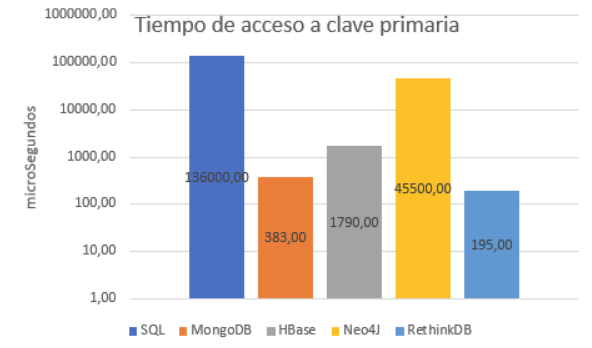
\includegraphics{grafico1.png}

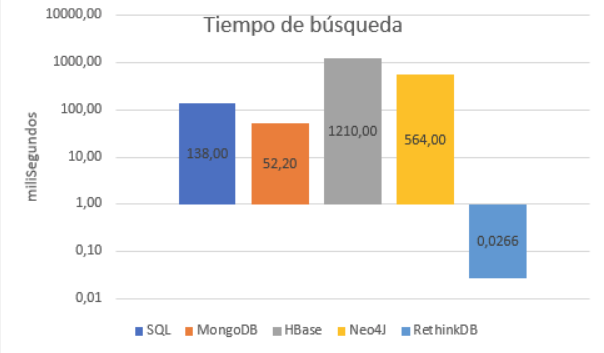
\includegraphics{grafico2.png}

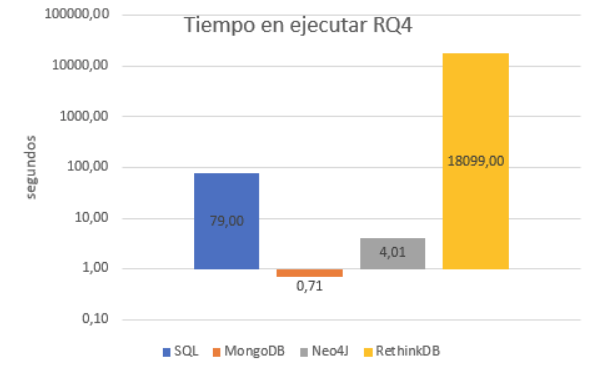
\includegraphics{grafico3.png}

    Nótese como RethinkDB supera a sus competidores en las dos primeras
pruebas. Sin embargo, en una consulta tan ``compleja'' como la RQ4, el
tiempo de ejecución se dispara a más de 5 horas.


    % Add a bibliography block to the postdoc
    
    
    
    \end{document}
